%!TEX program = xelatex
%!TEX root = ../../theory.tex

\documentclass[a4paper, openany, oneside]{memoir}
\usepackage[no-math]{fontspec}
\usepackage{pgfplots}
\pgfplotsset{compat=newest}
\usepackage{commath}
\usepackage{mathtools}
\usepackage{amssymb}
\usepackage{amsthm}
\usepackage{booktabs}
\usepackage{mathtools}
\usepackage{xcolor}
\usepackage[separate-uncertainty=true, per-mode=symbol]{siunitx}
\usepackage[noabbrev, capitalize]{cleveref}
\usepackage{listings}
\usepackage[american inductor, european resistor]{circuitikz}
\usepackage{amsmath}
\usepackage{amsfonts}
\usepackage{ifxetex}
\usepackage[dutch,english]{babel}
\usepackage[backend=bibtexu,texencoding=utf8,bibencoding=utf8,style=ieee,sortlocale=en_GB,language=auto]{biblatex}
\usepackage[strict,autostyle]{csquotes}
\usepackage{parskip}
\usepackage{import}
\usepackage{standalone}
\usepackage{hyperref}
%\usepackage[toc,title,titletoc]{appendix}

\ifxetex{} % Fonts laden in het geval dat je met Xetex compiled
    \usepackage{fontspec}
    \defaultfontfeatures{Ligatures=TeX} % To support LaTeX quoting style
    \setromanfont{Palatino Linotype} % Tover ergens in Font mapje in root.
    \setmonofont{Source Code Pro}
\else % Terug val in standaard pdflatex tool chain. Geen ondersteuning voor OTT fonts
    \usepackage[T1]{fontenc}
    \usepackage[utf8]{inputenc}
\fi
\newcommand{\references}[1]{\begin{flushright}{#1}\end{flushright}}
\renewcommand{\vec}[1]{\boldsymbol{\mathbf{#1}}}
\newcommand{\uvec}[1]{\boldsymbol{\hat{\vec{#1}}}}
\newcommand{\mat}[1]{\boldsymbol{\mathbf{#1}}}
\newcommand{\fasor}[1]{\boldsymbol{\tilde{\vec{#1}}}}
\newcommand{\cmplx}[0]{\mathrm{j}}
\renewcommand{\Re}[0]{\operatorname{Re}}
\newcommand{\Cov}{\operatorname{Cov}}
\newcommand{\Var}{\operatorname{Var}}
\newcommand{\proj}{\operatorname{proj}}
\newcommand{\Perp}{\operatorname{perp}}
\newcommand{\col}{\operatorname{col}}
\newcommand{\rect}{\operatorname{rect}}
\newcommand{\sinc}{\operatorname{sinc}}
\newcommand{\IT}{\operatorname{IT}}
\newcommand{\F}{\mathcal{F}}

\newtheorem{definition}{Definition}
\newtheorem{theorem}{Theorem}


\DeclareSIUnit{\voltampere}{VA} %apparent power
\DeclareSIUnit{\pii}{\ensuremath{\pi}}

\hypersetup{%setup hyperlinks
    colorlinks,
    citecolor=black,
    filecolor=black,
    linkcolor=black,
    urlcolor=black
}

% Example boxes
\usepackage{fancybox}
\usepackage{framed}
\usepackage{adjustbox}
\newenvironment{simpages}%
{\AtBeginEnvironment{itemize}{\parskip=0pt\parsep=0pt\partopsep=0pt}
\def\FrameCommand{\fboxsep=.5\FrameSep\shadowbox}\MakeFramed{\FrameRestore}}%
{\endMakeFramed}

% Impulse train
\DeclareFontFamily{U}{wncy}{}
\DeclareFontShape{U}{wncy}{m}{n}{<->wncyr10}{}
\DeclareSymbolFont{mcy}{U}{wncy}{m}{n}
\DeclareMathSymbol{\Sha}{\mathord}{mcy}{"58}
\addbibresource{../../../../includes/bibliography.bib}

\begin{document}
\section{Preliminaries}

Vectors are denoted by lower-case bold-faced letters and matrices are denoted by upper-case bold-faced letters. Unless stated otherwise, a vector is always assumed to be a column vector. The complex conjugate of a vector $\vec{x}$ is denoted by $\bar{\vec{x}}$. The inner product of an inner product space is denoted by $\cdot$. We now introduce notation to denote elements of vectors and matrices.

\begin{blockDefinition}[Vector Element]
    Let $\vec{x} \in \mathbb{C}^N$. Then $(\vec{x})_i$ denotes the $i$'th element of $\vec{x}$ for $i = 1,\ldots,N$.
\end{blockDefinition}

\begin{blockDefinition}[Matrix Element]
    Let $\mat{A}$ be an $M \times N$ matrix. Then $(\mat{A})_{i,j}$ denotes the $j$'th element of the $i$'th row of $\mat{A}$ for $i = 1,\ldots,M$ and $j=1,\ldots,N$.
\end{blockDefinition}

\begin{blockDefinition}
    Let $\vec{x} \in \{1\}^N$. Then $\vec{1}_N$ denotes $\vec{x}$.
\end{blockDefinition}

We also need notation to denote two uncommon operations.

\begin{blockDefinition}[Subvector]
    Let $\vec{x} \in \mathbb{C}^N$. Then $\vec{x}[a,b]$ denotes a vector $\vec{z} \in \mathbb{C}^{b-a+1}$ such that $(\vec{z})_i = (\vec{x})_{i+a-1}$ for $i = 1,\ldots,b-a+1$.
\end{blockDefinition}

\begin{blockDefinition}[Submatrix]
    Let $\mat{A}$ be an $M \times N$ matrix. Then $\mat{A}[a,b]$ denotes the $M \times b-a+1$ matrix $\mat{B}$ such that $(\mat{B})_{i,j}=(\mat{A})_{i,j+a-1}$ for $i = 1,\ldots,M$ and $j = 1,\ldots,b-a+1$.
\end{blockDefinition}

Subvectors and submatrices are found in MATLAB in a very similar way. For example, if \texttt{x} represents a vector $\vec{x}$ in MATLAB, then \texttt{x(a:b)} is equivalent to $\vec{x}[a,b]$. Note that subvectors and submatrices include both boundary elements.
% \begin{blockDefinition}[Reverse of Vector]
%     Let $\vec{x} \in \mathbb{C}^N$. Then the reverse of $\vec{x}$ denotes a vector $\vec{y} \in \mathbb{C}^N$ such that $(\vec{y})_i = (\vec{x})_{N-i+1}$ for $i = 1,\ldots,N$.
% \end{blockDefinition}
We now define the convolution operator as a closed binary operation on vectors. The definition is similar to the definition of convolution for discrete signals. This implies that results similar to well-known theorems can be obtained.

\begin{blockDefinition}[Convolution]
    Let $\vec{x} \in \mathbb{C}^N$ and $\vec{y} \in \mathbb{C}^M$. Then $\vec{x} \ast \vec{y}$ denotes a vector $\vec{z} \in \mathbb{C}^{N+M-1}$ such that
    \begin{align*}
        (\vec{z})_i = \sum_{k=1}^{N} (\vec{x})_k (\vec{y})_{i-k+1}
    \end{align*}
    where $(\vec{x})_i=0$ for $i \le 0$ and $i \ge N+1$ and $(\vec{y})_i=0$ for $i \le 0$ and $i \ge M+1$.
\end{blockDefinition}

\cref{fig:vis-convolution} depicts the convolution operator.

\begin{figure}
    \centering
    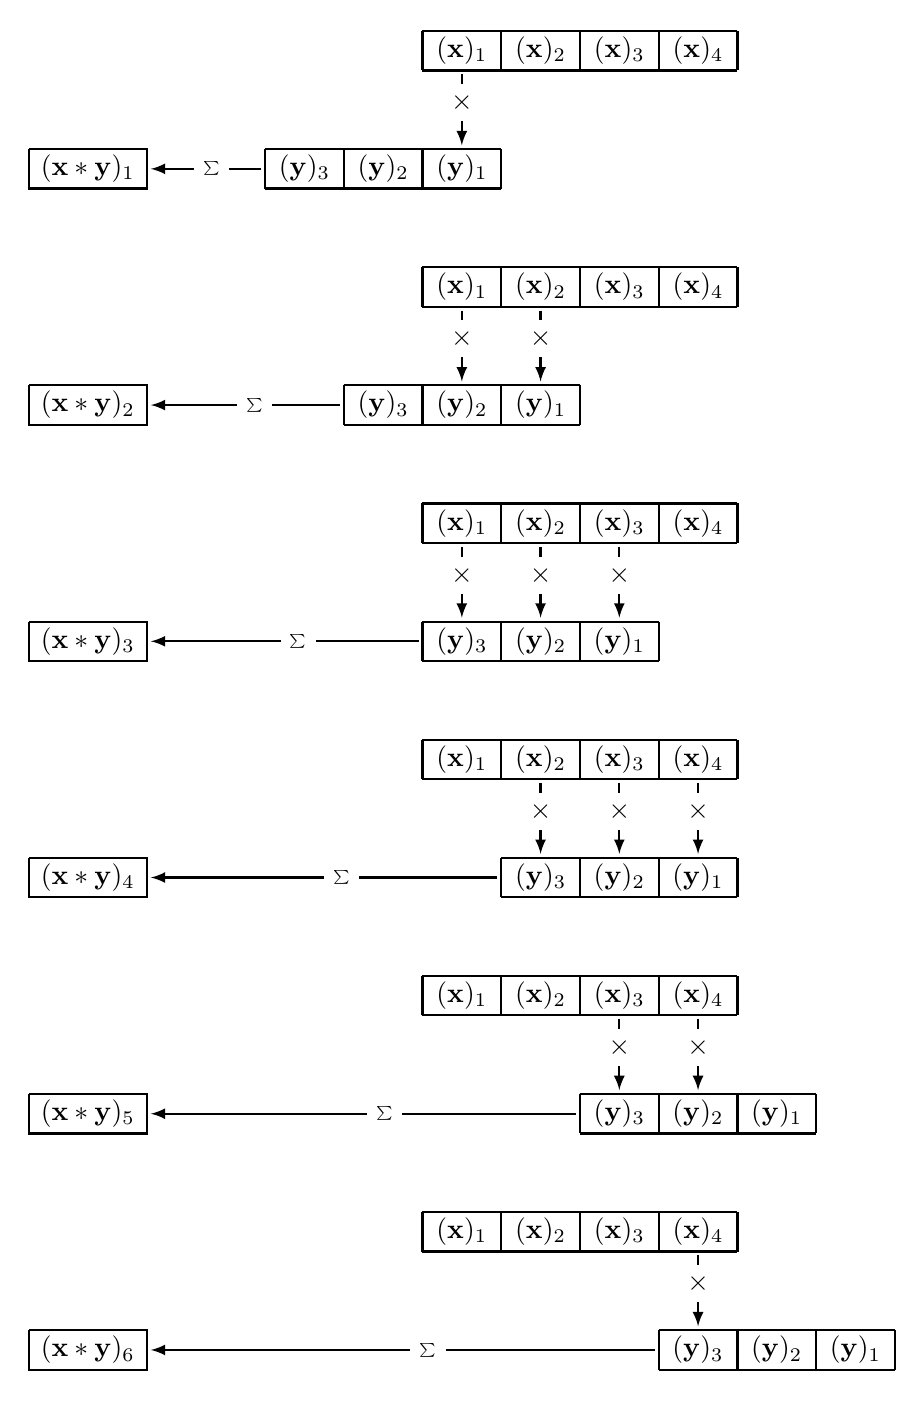
\begin{tikzpicture}
        \newcommand{\drawitem}[3]{
            \begin{scope}[shift={(0,#1*-3)}]
                \draw [black, thick] (0,0.5) -- (4,0.5);
                \draw [black, thick] (0,0) -- (4,0);

                \draw [black, thick] (-2+#1-1,-1) -- (1+#1-1,-1);
                \draw [black, thick] (-2+#1-1,-1.5) -- (1+#1-1,-1.5);
                \foreach \i in {0,...,4} {
                    \draw [black, thick] (\i, 0) -- (\i, 0.5);
                }
                \foreach \i in {1,...,4} {
                    \draw ({\i-0.5},0.25) node[black] {$(\vec{x})_{\i}$};
                }

                \foreach \i in {-2,...,1} {
                    \draw [black, thick] (\i+#1-1, -1) -- (\i+#1-1, -1.5);
                }
                \foreach \i in {1,...,3} {
                    \draw ({(4-\i)-2.5+#1-1},-1.25) node[black] {$(\vec{y})_{\i}$};
                }

                \foreach \i in {#2,...,#3} {
                    \draw [black, thick, >=latex, ->] (\i+0.5,-0.05) -- node[pos=0.4,fill=white] {$\times$} (\i+0.5,-0.95);
                }
                \draw [black, thick, >=latex, ->] (-2.05+#1-1,-1.25) -- node[pos=0.45,fill=white] {\tiny$\sum$} (-3.45,-1.25);
                \draw [black, thick] (-5,-1) -- (-5,-1.5) -- (-3.5,-1.5) -- (-3.5,-1) -- (-5,-1);
                \draw (-4.25,-1.25) node[black] {$(\vec{x} \ast \vec{y})_{#1}$};
            \end{scope}
        }
        \drawitem{1}{0}{0}
        \drawitem{2}{0}{1}
        \drawitem{3}{0}{2}
        \drawitem{4}{1}{3}
        \drawitem{5}{2}{3}
        \drawitem{6}{3}{3}
    \end{tikzpicture}
    \caption{Visualisation of $\vec{x} \ast \vec{y}$ where $\vec{x} \in \mathbb{C}^4$ and $\vec{y} \in \mathbb{C}^3$}
    \label{fig:vis-convolution}
\end{figure}

\begin{blockTheorem}[Commutativity of Convolution] \label{th:conv-comm}
    Let $\vec{x} \in \mathbb{C}^N$ and $\vec{y} \in \mathbb{C}^M$. Then $\vec{x} \ast \vec{y} = \vec{y} \ast \vec{x}$.
\end{blockTheorem}

The proof of \cref{th:conv-comm} will be given in \cref{sec:proofs}. We also define correlation as a closed binary operation on vectors. The definition is again similar to the definition of correlation for discrete signals.

\begin{blockDefinition}[Deterministic Cross-correlation]
    Let $\vec{x} \in \mathbb{C}^N$ and $\vec{y} \in \mathbb{C}^M$. Then $\vec{x} \circ \vec{y}$ denotes a vector $\vec{z} \in \mathbb{C}^{N+M-1}$ such that
    \begin{align*}
        (\vec{z})_i = \sum_{k=1}^{N} (\vec{x})_k (\conj{\vec{y}})_{M-i+k}
    \end{align*}
    where $(\vec{x})_i=0$ for $i \le 0$ and $i \ge N+1$ and $(\vec{y})_i=0$ for $i \le 0$ and $i \ge M+1$.
\end{blockDefinition}

\cref{fig:vis-correlation} depicts the correlation operator. Notice that the operation of the correlation operator is similar to the operation of the convolution operator.

\begin{figure}
    \centering
    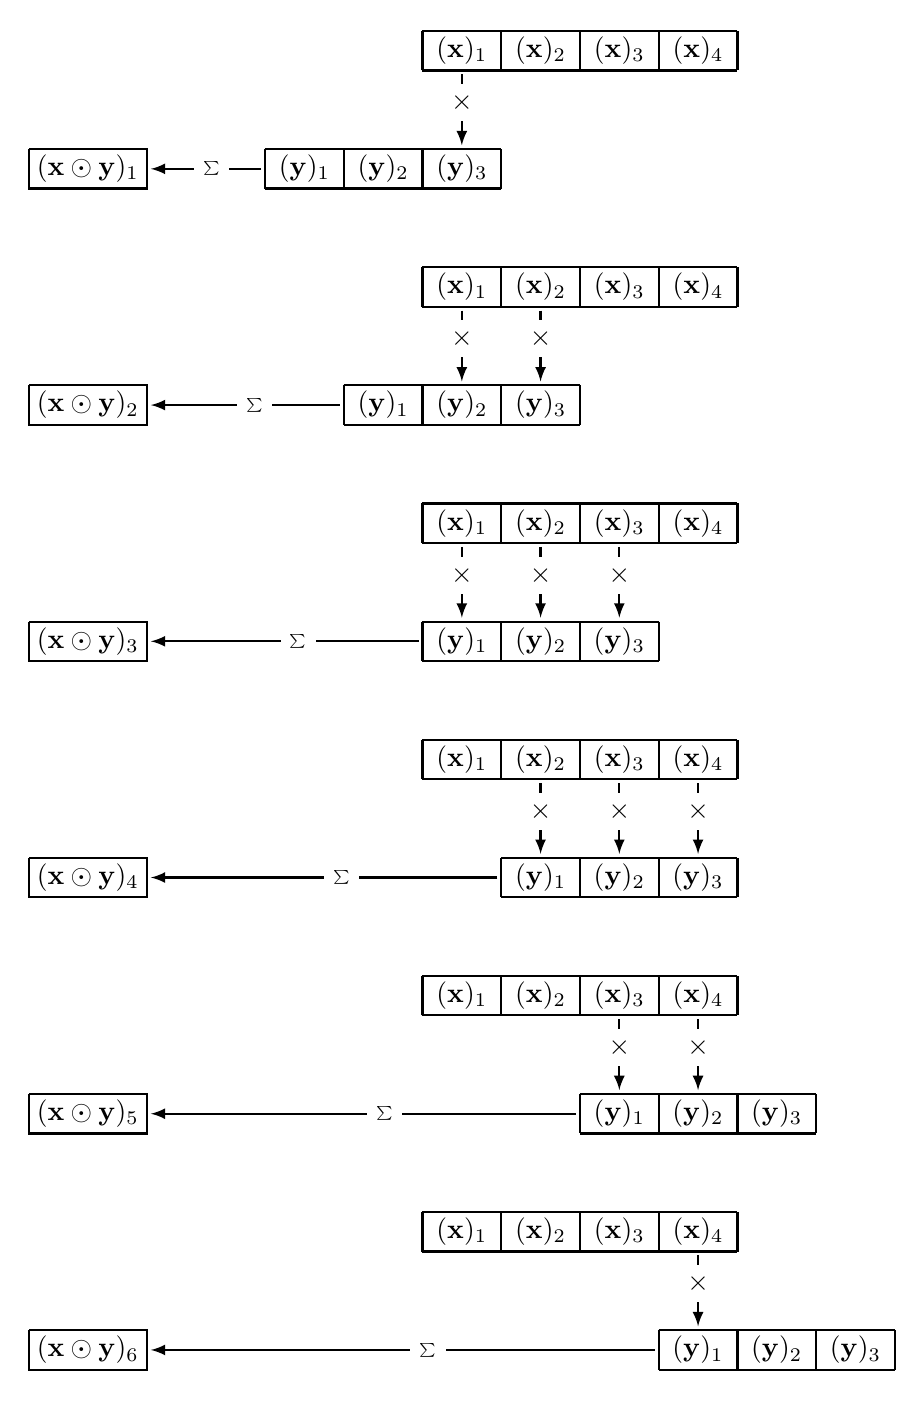
\begin{tikzpicture}
        \newcommand{\drawitem}[3]{
            \begin{scope}[shift={(0,#1*-3)}]
                \draw [black, thick] (0,0.5) -- (4,0.5);
                \draw [black, thick] (0,0) -- (4,0);

                \draw [black, thick] (-2+#1-1,-1) -- (1+#1-1,-1);
                \draw [black, thick] (-2+#1-1,-1.5) -- (1+#1-1,-1.5);
                \foreach \i in {0,...,4} {
                    \draw [black, thick] (\i, 0) -- (\i, 0.5);
                }
                \foreach \i in {1,...,4} {
                    \draw ({\i-0.5},0.25) node[black] {$(\vec{x})_{\i}$};
                }

                \foreach \i in {-2,...,1} {
                    \draw [black, thick] (\i+#1-1, -1) -- (\i+#1-1, -1.5);
                }
                \foreach \i in {1,...,3} {
                    \draw ({\i-2.5+#1-1},-1.25) node[black] {$(\vec{y})_{\i}$};
                }

                \foreach \i in {#2,...,#3} {
                    \draw [black, thick, >=latex, ->] (\i+0.5,-0.05) -- node[pos=0.4,fill=white] {$\times$} (\i+0.5,-0.95);
                }
                \draw [black, thick, >=latex, ->] (-2.05+#1-1,-1.25) -- node[pos=0.45,fill=white] {\tiny$\sum$} (-3.45,-1.25);
                \draw [black, thick] (-5,-1) -- (-5,-1.5) -- (-3.5,-1.5) -- (-3.5,-1) -- (-5,-1);
                \draw (-4.25,-1.25) node[black] {$(\vec{x} \odot \vec{y})_{#1}$};
            \end{scope}
        }
        \drawitem{1}{0}{0}
        \drawitem{2}{0}{1}
        \drawitem{3}{0}{2}
        \drawitem{4}{1}{3}
        \drawitem{5}{2}{3}
        \drawitem{6}{3}{3}
    \end{tikzpicture}
    \caption{Visualisation of $\vec{x} \odot \vec{y}$ where $\vec{x} \in \mathbb{C}^4$ and $\vec{y} \in \mathbb{C}^3$}
    \label{fig:vis-correlation}
\end{figure}


It is important to notice that the convolution operator and deterministic cross-correlation operator are equivalent to respectively the functions \texttt{conv} and \texttt{xcorr} in MATLAB. We furthermore define the Hadamard product as a closed binary operation on vectors.

\begin{blockDefinition}[Hadamard Product]
    Let $\vec{x} \in \mathbb{C}^N$ and $\vec{y} \in \mathbb{C}^N$. Then $\vec{x} \odot \vec{y}$ denotes a vector $\vec{z} \in \mathbb{C}^N$ such that $(\vec{z})_i = (\vec{x})_i (\vec{y})_i$ for $i = 1,\ldots,N$.
\end{blockDefinition}

Note that $\odot$ is similar to $\cdot$. This similarity makes sense, since the inner product and Hadamard product are closely related. Also, the Hadamard product is equivalent to element-wise multiplication in MATLAB.
The following theorem identifies the expected value of the correlation operator.

\begin{blockTheorem} \lab{th:correlation-bias}
    Let $X[n]$ and $Y[n]$ be wide sense stationary stochastic processes. Let $\vec{x} \in \mathbb{C}^N$ and $\vec{y} \in \mathbb{C}^M$ be such that $(\vec{x})_i = X[i]$ for $i=1,\ldots,N$ and $(\vec{y})_i = Y[i]$ for $i=1,\ldots,M$.  Then $(\vec{x} \circ \vec{y})_{i+M}$ is an unbiased estimator of $W[i]R_{X,Y}[i]$ where
    \begin{align*}
        W[i] = \begin{cases}
            M + i & \text{if } -M + 1 \le i \le -M + K, \\
            K & \text{if } -M + K < i < N - K, \\
            N - i & \text{if } N - K \le i \le N - 1, \\
            0 & \text{elsewhere,}
        \end{cases}
    \end{align*}
    and $K = \min\{N,M\}$.
\end{blockTheorem}

\cref{th:correlation-bias} shows that the correlation operator is a biased estimator of the cross-correlation. \cref{fig:vis-wi} visualises this bias.

\begin{figure}
    \centering
    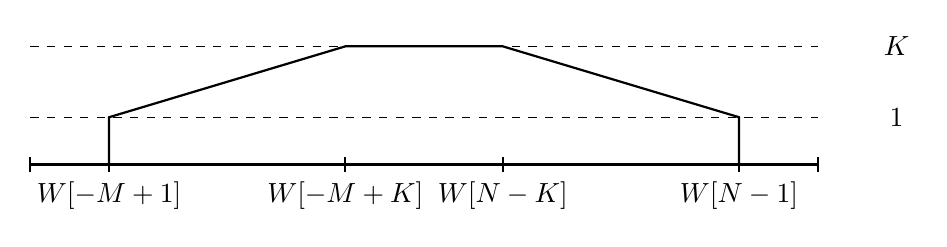
\begin{tikzpicture}
        \draw [thick,black] (-5,0) -- (5,0);
        \draw [thick,black] (-5,-0.1) -- (-5,0.1);
        \draw [thick,black] (5,-0.1) -- (5,0.1);
        \draw [thick,black] (1,-0.1) -- (1,0.1);
        \draw [thick,black] (-1,-0.1) -- (-1,0.1);
        \draw [thick,black] (-4,0.1) -- (-4,-0.1);
        \draw [thick,black] (4,-0.1) -- (4,0.1);
        \draw [dashed] (-5,0.6) -- (5,0.6);
        \draw [black,thick] (-4,0) -- (-4,0.6) -- (-1,1.5) -- (1,1.5) -- (4,0.6) -- (4,0);
        \draw [dashed] (-5,1.5) -- (5,1.5);
        \draw (6,1.5) node[black] {$K$};
        \draw (6,0.6) node[black] {$1$};
        \draw (-4,-0.4) node[black] {$W[-M+1]$};
        \draw (-1,-0.4) node[black] {$W[-M+K]$};
        \draw (1,-0.4) node[black] {$W[N-K]$};
        \draw (4,-0.4) node[black] {$W[N-1]$};
    \end{tikzpicture}
    \caption{Visualisation of $W[i]$ from \cref{th:correlation-bias}}
    \label{fig:vis-wi}
\end{figure}

Finally, we extend the use of dots to denote finite sequences.

\begin{blockDefinition} \lab{def:dots-extended}
    Let $N \in \mathbb{N}$. Then $(1,1),\ldots,(N,N)$ denotes the sequence

    \makebox[\textwidth]{\centering
        $(1,1),\ldots(1,N),(2,1),\ldots,(2,N),(3,1),\ldots,(N,N).$
    } \nolinebreak
\end{blockDefinition}
\end{document}